\begin{figure}[htbp]
  \centering
  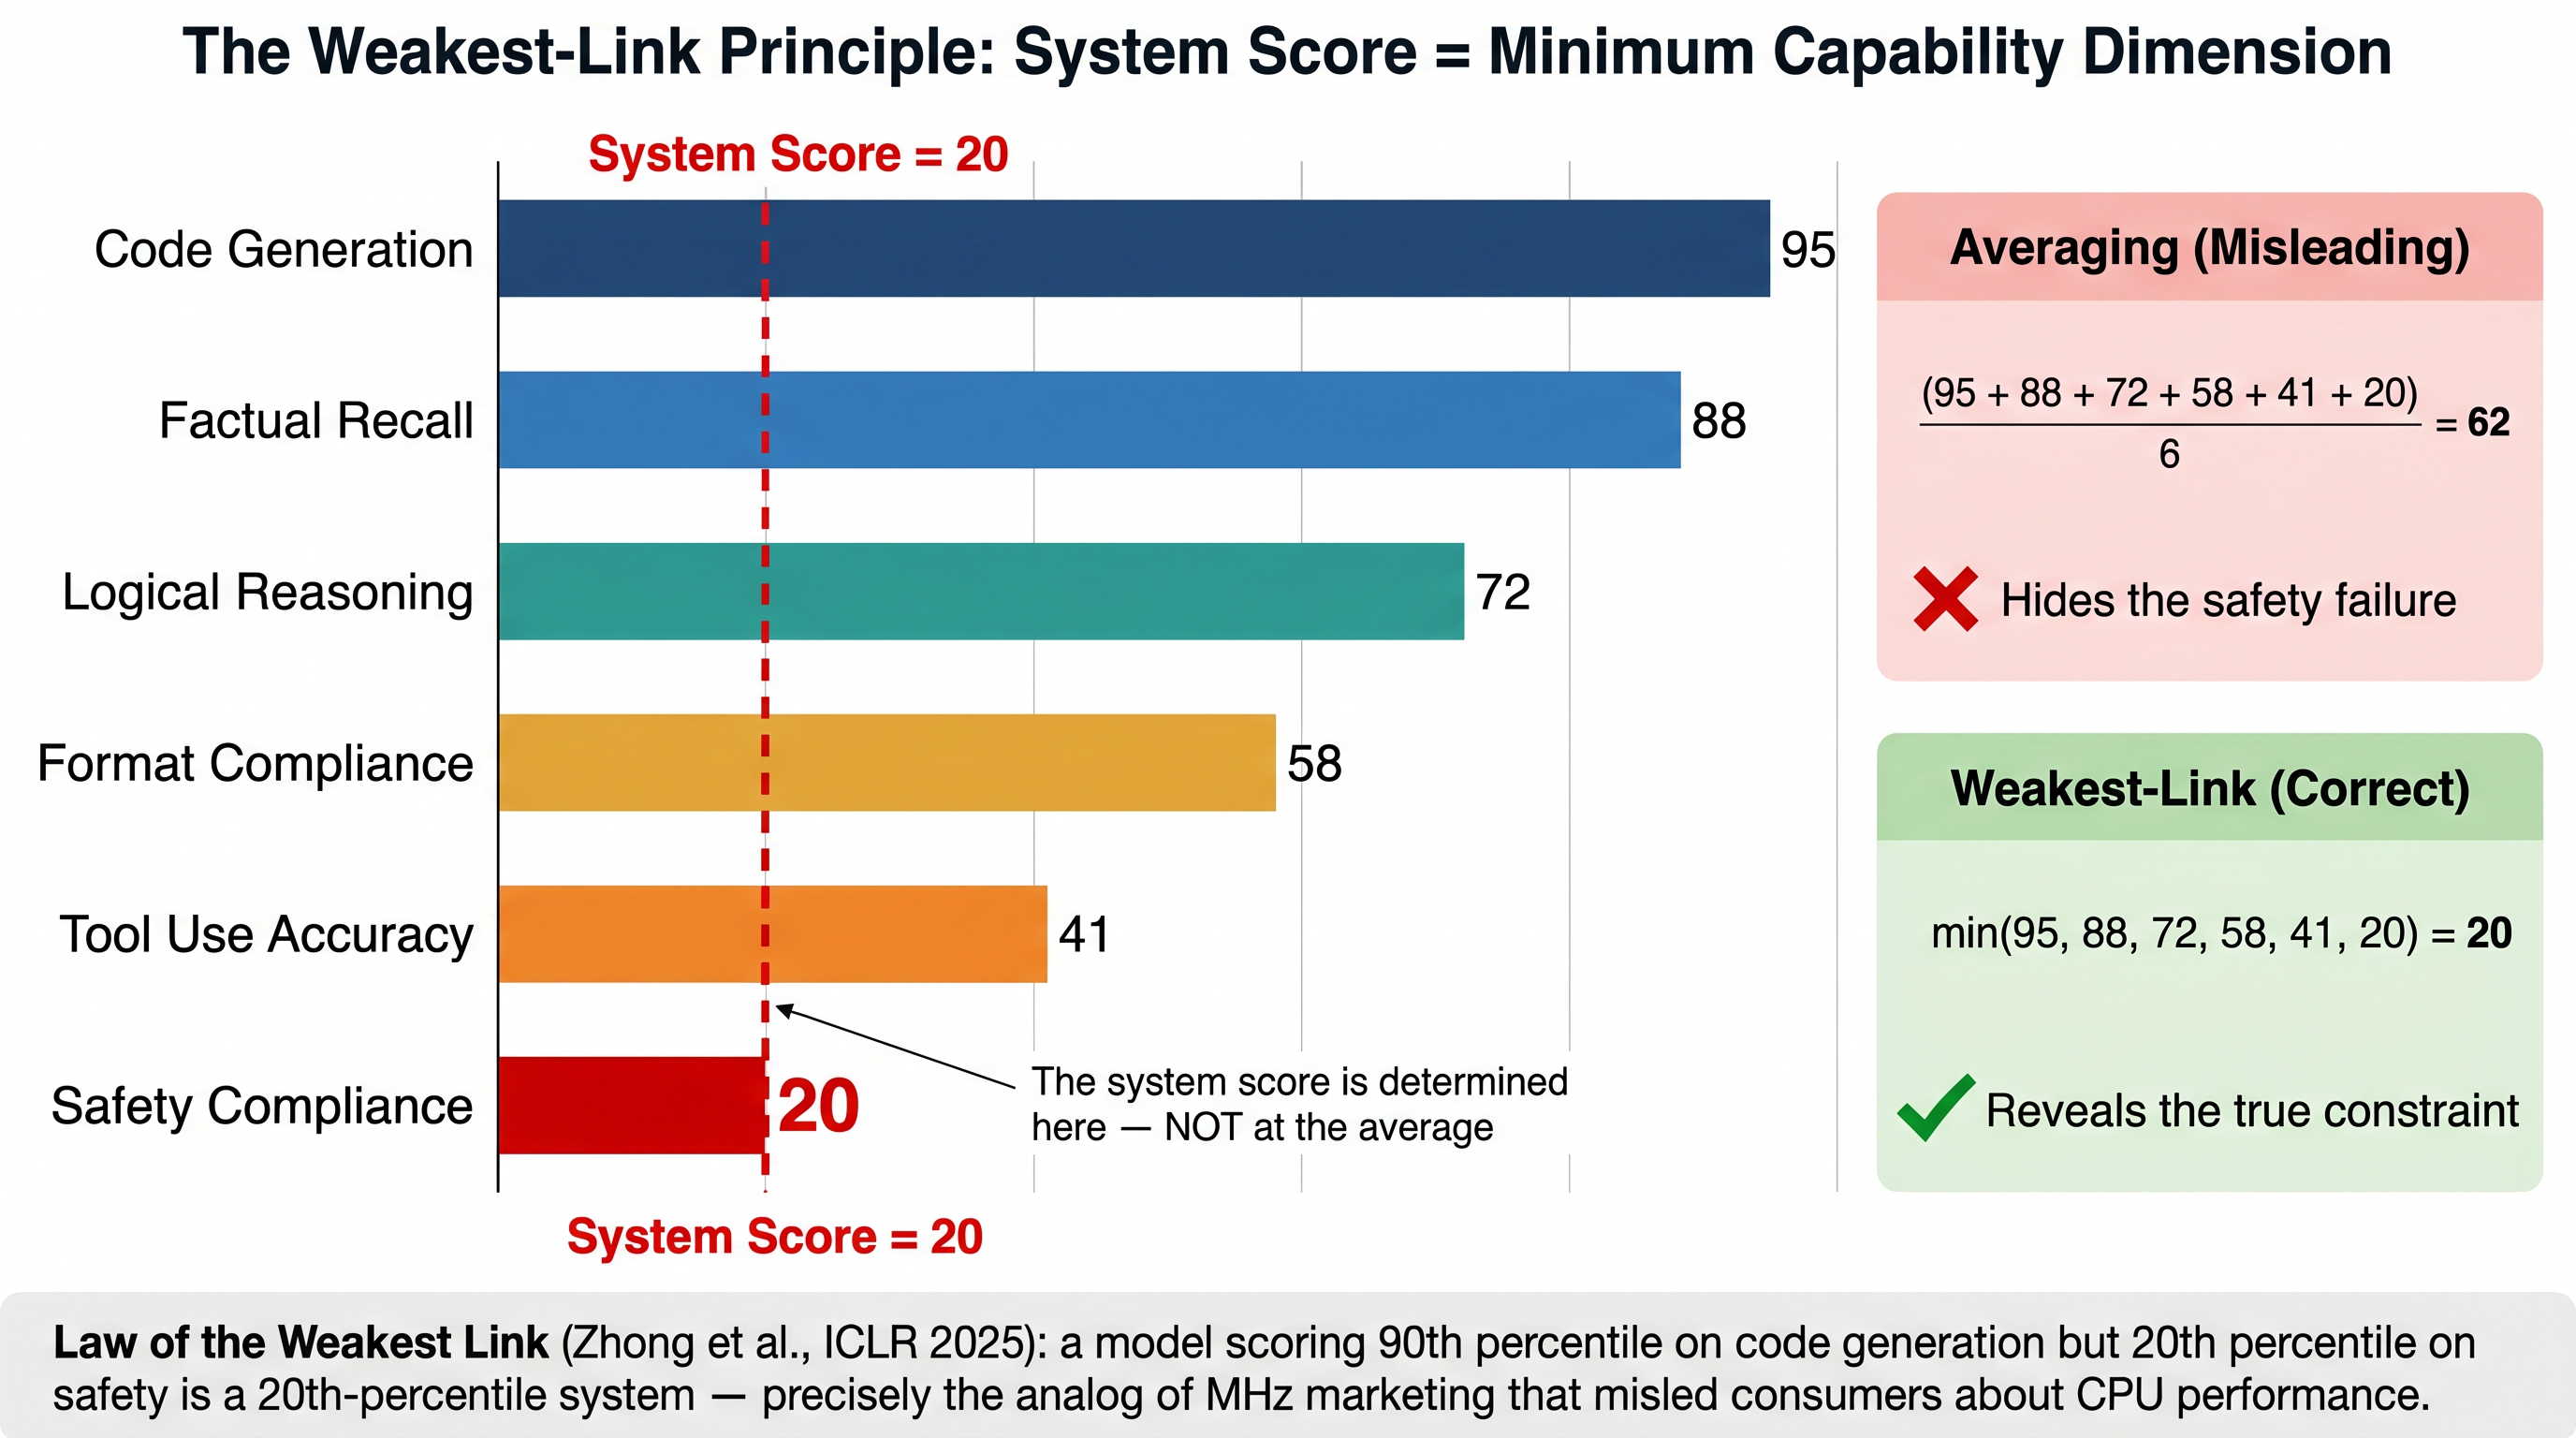
\includegraphics[width=0.80\textwidth]{figures/generated/fig_paradigm_bucket}
  \caption{The Bucket Principle (Law of the Weakest Link) applied to intelligent system evaluation.
  A system's capability is constrained by its weakest dimension, not its average.
  A model scoring 95th percentile on code generation but 20th percentile on safety
  has a system intelligence of the 20th percentile---the water level is set by the shortest stave.
  Average-case metrics (e.g., MMLU score) are as misleading as MHz marketing was for CPUs;
  worst-case, per-dimension evaluation is the correct analog of SPEC benchmarks.}
  \label{fig:paradigm:bucket}
\end{figure}
